\section{Durchführung}
\label{sec:Durchführung}
\begin{figure}
  \centering
  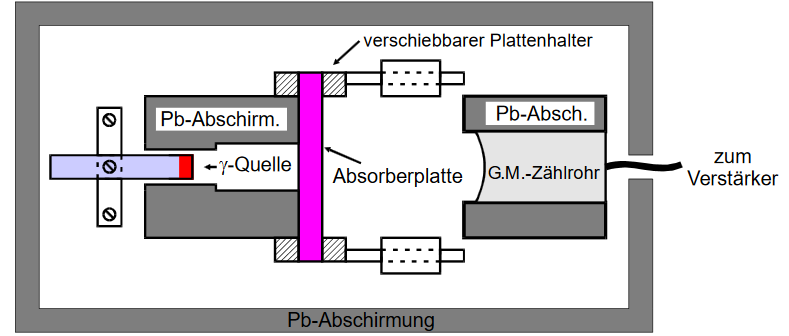
\includegraphics[width=0.6\textwidth]{aufbau.PNG}
  \caption{Darstellung der Messaparatur.\cite{sample}}
  \label{fig:aufbau}
\end{figure}
In Abbildung \ref{fig:aufbau} ist der schematische Aufbau der Apparatur zu sehen.
Bei der Nullmessung wird über einen Zeitraum von $900\si{\second}$ die Hintergrundstahlung mittels
Geiger-Müller-Zählrohr und Impulszähler registriert.
Für die eigentliche Messung werden ein $\gamma$- und $\beta$-Strahler vor das Zählrohr gesetzt. Als Absorber
dienen verschiedene Materialien unterschiedlicher Dicke, diese werden zwischen Quelle und Zählrohr plaziert.
Die Zählzeit wird je nach Dicke des Asorbers angepasst.
Als $\gamma$-Strahler wird $^{137}$Cs verwendet und als $\beta$-Strahler $^{99}$Tc.
